


\tikzset{every picture/.style={line width=0.75pt}} %set default line width to 0.75pt        

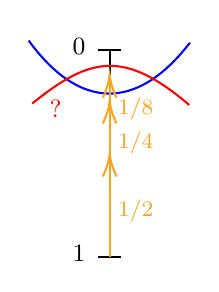
\begin{tikzpicture}[x=0.75pt,y=0.75pt,yscale=-1,xscale=1]
%uncomment if require: \path (0,534); %set diagram left start at 0, and has height of 534

%Straight Lines [id:da8648942484395017] 
\draw    (590.4,100.4) -- (590.4,200.07) ;
\draw [shift={(590.4,200.07)}, rotate = 270] [color={rgb, 255:red, 0; green, 0; blue, 0 }  ][line width=0.75]    (0,5.59) -- (0,-5.59)   ;
\draw [shift={(590.4,100.4)}, rotate = 270] [color={rgb, 255:red, 0; green, 0; blue, 0 }  ][line width=0.75]    (0,5.59) -- (0,-5.59)   ;
%Curve Lines [id:da5356270327996431] 
\onslide<10->{\draw [color={rgb, 255:red, 0; green, 0; blue, 255 }  ,draw opacity=1 ]   (551.4,95.73) .. controls (575.4,128.73) and (603.07,130.4) .. (629.07,96.73) ;}
%Straight Lines [id:da42007517029648045] 
\onslide<11->{\draw [color={rgb, 255:red, 245; green, 166; blue, 35 }  ,draw opacity=1 ]   (590.4,200.07) -- (590.4,152.23) ;
\draw [shift={(590.4,150.23)}, rotate = 90] [color={rgb, 255:red, 245; green, 166; blue, 35 }  ,draw opacity=1 ][line width=0.75]    (10.93,-3.29) .. controls (6.95,-1.4) and (3.31,-0.3) .. (0,0) .. controls (3.31,0.3) and (6.95,1.4) .. (10.93,3.29)   ;}
%Straight Lines [id:da4473125650369483] 
\onslide<12->{\draw [color={rgb, 255:red, 245; green, 166; blue, 35 }  ,draw opacity=1 ]   (590.4,150.23) -- (590.4,126.73) ;
\draw [shift={(590.4,124.73)}, rotate = 90] [color={rgb, 255:red, 245; green, 166; blue, 35 }  ,draw opacity=1 ][line width=0.75]    (10.93,-3.29) .. controls (6.95,-1.4) and (3.31,-0.3) .. (0,0) .. controls (3.31,0.3) and (6.95,1.4) .. (10.93,3.29)   ;}
%Straight Lines [id:da921748453412278] 
\onslide<13->{\draw [color={rgb, 255:red, 245; green, 166; blue, 35 }  ,draw opacity=1 ]   (590.4,124.73) -- (590.4,114.23) ;
\draw [shift={(590.4,112.23)}, rotate = 90] [color={rgb, 255:red, 245; green, 166; blue, 35 }  ,draw opacity=1 ][line width=0.75]    (10.93,-3.29) .. controls (6.95,-1.4) and (3.31,-0.3) .. (0,0) .. controls (3.31,0.3) and (6.95,1.4) .. (10.93,3.29)   ;}
%Curve Lines [id:da40449977786973723] 
\onslide<15->{\draw [color={rgb, 255:red, 255; green, 0; blue, 0 }  ,draw opacity=1 ]   (553.07,126.07) .. controls (581.4,103.07) and (597.73,100.4) .. (628.73,126.73) ;}

% Text Node
\draw (571,93) node [anchor=north west][inner sep=0.75pt]  [font=\small]  {$0$};
% Text Node
\draw (571,193) node [anchor=north west][inner sep=0.75pt]  [font=\small]  {$1$};
% Text Node
\onslide<10->{\draw (596,90) node [anchor=north west][inner sep=0.75pt]  [font=\small,color={rgb, 255:red, 0; green, 0; blue, 255 }  ,opacity=1 ]  {$\taumax$};}
% Text Node
\onslide<11->{\draw (593,171) node [anchor=north west][inner sep=0.75pt]  [font=\footnotesize,color={rgb, 255:red, 245; green, 166; blue, 35 }  ,opacity=1 ]  {$1/2$};}
% Text Node
\onslide<12->{\draw (593,138) node [anchor=north west][inner sep=0.75pt]  [font=\footnotesize,color={rgb, 255:red, 245; green, 166; blue, 35 }  ,opacity=1 ]  {$1/4$};}
% Text Node
\onslide<13->{\draw (593,122) node [anchor=north west][inner sep=0.75pt]  [font=\footnotesize,color={rgb, 255:red, 245; green, 166; blue, 35 }  ,opacity=1 ]  {$1/8$};}
% Text Node
\onslide<15->{\draw (560,123) node [anchor=north west][inner sep=0.75pt]  [font=\small,color={rgb, 255:red, 255; green, 0; blue, 0 }  ,opacity=1 ] [align=left] {?};}


\end{tikzpicture}
